
CMake通过三个阶段构建解决方案——配置、生成和运行构建工具。通常,在配置阶段就有了所有所需的数据。但每隔一段时间,我们就会遇到先有鸡还是先有蛋的问题。举一个前一节的例子——一个目标需要知道另一个目标的二进制工件的路径。但是,只有在解析所有列表文件并完成配置阶段之后,这些信息才可用。

该如何处理这种问题呢?可以为该信息创建一个占位符,并将其评估推迟到下一个阶段——生成阶段。

这就是生成器表达式(有时称为genexes)所做的事,其是围绕目标属性构建的,如LINK\_LIBRARIES、INCLUDE\_DIRECTORIES、COMPILE\_DEFINITIONS、传播属性和许多其他属性,但不是全部。遵循类似条件语句和变量求值的规则。

值得注意的是,表达式通常是在使用的目标上下文中求值的(除非另有明确说明)。

\begin{tcolorbox}[colback=blue!5!white,colframe=blue!75!black,title=重要的Note]
生成器表达式将在生成阶段计算(当配置完成并创建构建系统时),所以不能将其输出捕获到变量中,并打印到控制台。要调试它们,可以使用以下方法中的任何一种:

\begin{itemize}
\item 
将其写入一个文件(file()指令的这个特定版本支持生成器表达式):
\begin{lstlisting}[style=styleCMake]
file(GENERATE OUTPUT filename CONTENT "$<...>")
\end{lstlisting}

\item 
添加一个自定义目标,并从命令行显式地构建它:
\begin{lstlisting}[style=styleCMake]
custom_target(gendbg COMMAND ${CMAKE_COMMAND} -E echo "$<...>")
\end{lstlisting}
\end{itemize}
\end{tcolorbox}

\subsubsubsection{4.4.1\hspace{0.2cm}一般语法}

举一个最简单的例子:

\begin{lstlisting}[style=styleCMake]
target_compile_definitions(foo PUBLIC
	BAR=$<TARGET_FILE:foo>)
\end{lstlisting}

上面的命令在编译器的参数中添加了一个-D定义标志(暂时忽略PUBLIC),将BAR预处理器定义设置为foo目标的二进制工件的路径。

生成器表达式如何形成的?

\begin{center}
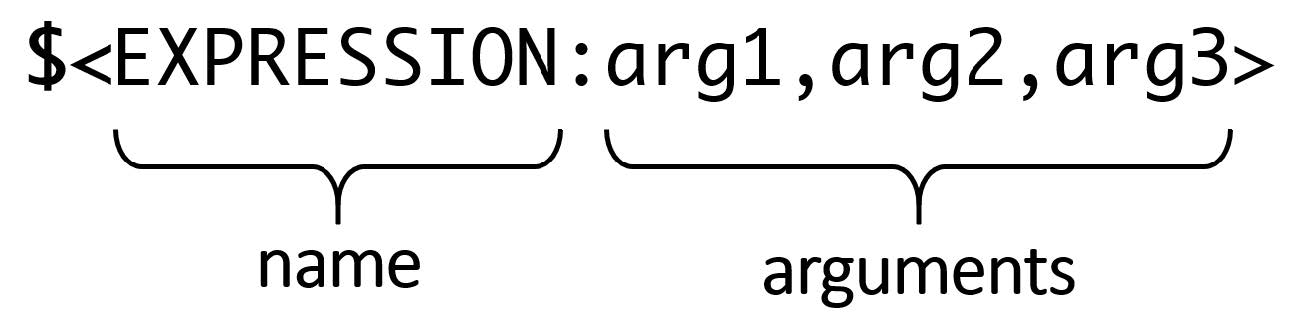
\includegraphics[width=0.5\textwidth]{content/2/chapter4/images/4.jpg}\\
图4.4 生成器表达式的语法
\end{center}

如图4.4所示,该结构看起来相当简单且可读:

\begin{itemize}
\item 
以\$和括号(\$<)开头

\item 
添加EXPRESSION名称

\item 
如果表达式需要参数,则添加冒号(:)并提供arg1、arg2和arg3值,用逗号分隔。

\item 
用>关闭表达式。
\end{itemize}

甚至有些表达式不需要任何参数,例如\$<PLATFORM\_ID>。然而,在使用生成器表达式更高级的特性时,生成器表达式很快就会变得非常混乱和复杂。

\hspace*{\fill} \\ %插入空行
\noindent
\textbf{嵌套}

将通用表达式作为参数传递给另一个表达式的能力开始,换句话说,通用表达式嵌套:

\begin{lstlisting}[style=styleCMake]
$<UPPER_CASE:$<PLATFORM_ID>>
\end{lstlisting}

这不是一个非常复杂的示例,但很容易想象当增加嵌套级别并使用使用多个参数的命令时会发生什么。

若这还不够,可以在组合中添加一个变量展开:

\begin{lstlisting}[style=styleCMake]
$<UPPER_CASE:${my_variable}>
\end{lstlisting}

在配置阶段将展开一个变量,生成阶段将展开一个生成表达式。这个功能有一些罕见的用法,但强烈建议别去使用。

\hspace*{\fill} \\ %插入空行
\noindent
\textbf{条件表达式}

生成器表达式支持布尔逻辑。这是一个很好的特性,但是由于历史原因,它的语法不一致,很难阅读。它有两种形式。第一种形式支持成功和失败的路径:

\begin{lstlisting}[style=styleCMake]
$<IF:condition,true_string,false_string>
\end{lstlisting}

这里的语法与所有其他表达式对齐,并且与所有表达式一样,允许嵌套。因此,可以用另一个表达式替换任何参数,并生成一些非常复杂的计算——甚至可以将一个条件嵌套在另一个条件中。这种形式恰好需要三个参数,因此不能省略任何内容。在未满足条件的情况下,跳过值的最佳选项如下:

\begin{lstlisting}[style=styleCMake]
$<IF:condition,true_string,>
\end{lstlisting}

第二种形式是前一种的缩写;只有满足以下条件,才会展开为字符串:

\begin{lstlisting}[style=styleCMake]
$<condition:true_string >
\end{lstlisting}

这打破了提供EXPRESSION名称作为第一个标记的惯例。我认为这里的意图是缩短表达并跳过这三个宝贵的字符,但结果真的很难合理解释。下面是CMake文档中的一个例子:

\begin{lstlisting}[style=styleCMake]
$<$<AND:$<COMPILE_LANGUAGE:CXX>,$<CXX_COMPILER_ID:AppleClan
	g,Clang>>:COMPILING_CXX_WITH_CLANG>
\end{lstlisting}

希望语法与常规if指令的条件一样,但遗憾的是事实并非如此。

\subsubsubsection{4.4.2\hspace{0.2cm}计算类型}

生成器表达式可以计算成两种类型——布尔或字符串。布尔值由1(真)和0(假)表示。其他的都只是一个字符串。

在条件表达式中作为条件传递的嵌套表达式,显式为布尔值。

有一个显式逻辑运算符可以将字符串转换为布尔类型,但布尔类型可以隐式转换为字符串。

现在我们知道了基本的语法,来看看能用它做什么。

\hspace*{\fill} \\ %插入空行
\noindent
\textbf{布尔型}

在前一节开始讨论条件表达式。这里先把整个概念讲完,这样以后就不需要再回头讲了。有三种类型的表达式的值为布尔值。

\hspace*{\fill} \\ %插入空行
\noindent
\textbf{逻辑运算符}

逻辑运算符有4种:

\begin{itemize}
\item 
\begin{lstlisting}[style=styleCMake]
$<NOT:arg> 
\end{lstlisting}

否定布尔参数。

\item 
\begin{lstlisting}[style=styleCMake]
$<AND:arg1,arg2,arg3...> 
\end{lstlisting}

若所有参数都为1,则返回1。

\item 
\begin{lstlisting}[style=styleCMake]
$<OR:arg1,arg2,arg3...> 
# returns 1 if any of the arguments is 1.
\end{lstlisting}

\item 
\begin{lstlisting}[style=styleCMake]
$<BOOL:string_arg> 
\end{lstlisting}

将参数从字符串转换为布尔类型。
\end{itemize}

若这些条件都不满足,字符串转换将计算为1:

\begin{itemize}
\item 
字符串为空。

\item 
字符串不区分大小写,相当于0、FALSE、OFF、N、NO、IGNORE或NOTFOUND。

\item 
字符串以-NOTFOUND后缀结尾(区分大小写)。
\end{itemize}

\hspace*{\fill} \\ %插入空行
\noindent
\textbf{字符串比较}

若满足条件比较的值为1,否则为0:

\begin{itemize}
\item 
\begin{lstlisting}[style=styleCMake]
$<STREQUAL:arg1,arg2> 
\end{lstlisting}

是区分大小写的字符串比较。

\item 
\begin{lstlisting}[style=styleCMake]
$<EQUAL:arg1,arg2> 
\end{lstlisting}

将字符串转换为数字并比较是否相等。

\item 
\begin{lstlisting}[style=styleCMake]
$<IN_LIST:arg,list> 
\end{lstlisting}

检查arg元素是否在列表列表中(区分大小写)。

\item 
\begin{lstlisting}[style=styleCMake]
$<VERSION_EQUAL:v1,v2>, $<VERSION_LESS:v1,v2>,
$<VERSION_GREATER:v1,v2>, $<VERSION_LESS_EQUAL:v1,v2>,
$<VERSION_GREATER_EQUAL:v1,v2> 
\end{lstlisting}
版本组件的比较。
\end{itemize}

\hspace*{\fill} \\ %插入空行
\noindent
\textbf{查询变量}

有许多变量包含布尔类型的值。如果满足条件,则求值为1,否则为0。

简单的查询:

\begin{itemize}
\item 
\begin{lstlisting}[style=styleCMake]
$<TARGET_EXISTS:arg> 
\end{lstlisting}
arg目标是否存在?
\end{itemize}

有多个查询扫描传递的参数以获取特定值:

\begin{itemize}
\item 
\begin{lstlisting}[style=styleCMake]
$<CONFIG:args>
\end{lstlisting}
是args中的当前配置(Debug, Release,等等)(不区分大小写)。

\item 
\begin{lstlisting}[style=styleCMake]
$<PLATFORM_ID:args>
\end{lstlisting}
是args中的当前平台ID。

\item 
\begin{lstlisting}[style=styleCMake]
$<LANG_COMPILER_ID:args>
\end{lstlisting}
是CMake的LANG编译器ID在args中,其中LANG是C、CXX、CUDA、OBJC、OBJCXX、Fortran或ISPC中的一种。

\item 
\begin{lstlisting}[style=styleCMake]
$<LANG_COMPILER_VERSION:args>
\end{lstlisting}
是CMake的LANG编译器的args版本,其中LANG是C、CXX、CUDA、OBJC、OBJCXX、Fortran或ISPC中的一种。

\item 
\begin{lstlisting}[style=styleCMake]
$<COMPILE_FEATURES:features>
\end{lstlisting}
若编译器支持此目标的特性,则返回true。

\item 
\begin{lstlisting}[style=styleCMake]
$<COMPILE_LANG_AND_ID:lang,compiler_id1,compiler_id2...>
\end{lstlisting}
是这个lang目标的语言,是在compiler\_ids列表中为这个目标使用的编译器。这个表达式对于指定特定编译器的配置细节很有用:

\begin{lstlisting}[style=styleCMake]
target_compile_definitions(myapp PRIVATE
	$<$<COMPILE_LANG_AND_ID:CXX,AppleClang,Clang>:CXX_CLANG>
	$<$<COMPILE_LANG_AND_ID:CXX,Intel>:CXX_INTEL>
	$<$<COMPILE_LANG_AND_ID:C,Clang>:C_CLANG>
)
\end{lstlisting}

在前面的例子中,若用AppleClang或Clang编译CXX编译器,则会设置-DCXX\_CLANG定义。对于来自Intel的CXX编译器,将设置-DCXX\_INTEL标志。最后,对于C和Clang编译器,我们将得到-DC\_CLANG定义。

\item 
\begin{lstlisting}[style=styleCMake]
$<COMPILE_LANGUAGE:args>
\end{lstlisting}

若使用一种语言在args中编译此目标。可以用来为编译器提供特定于语言的标志:

\begin{lstlisting}[style=styleCMake]
target_compile_options(myapp
	PRIVATE $<$<COMPILE_LANGUAGE:CXX>:-fno-exceptions>
)
\end{lstlisting}

若编译CXX,编译器将使用-fno-exceptions标志

\item 
\begin{lstlisting}[style=styleCMake]
$<LINK_LANG_AND_ID:lang,compiler_id1,compiler_id2...>
\end{lstlisting}

与COMPILE\_LANG\_AND\_ID的工作原理类似,但会检查链接步骤使用的语言。使用此表达式指定特定语言的链接库、链接选项、链接目录和链接依赖项,以及目标中的链接器组合。

\item 
\begin{lstlisting}[style=styleCMake]
$<LINK_LANGUAGE:args>
\end{lstlisting}

args中用于链接步骤的语言。
\end{itemize}

\hspace*{\fill} \\ %插入空行
\noindent
\textbf{字符串的求值}

有很多表达式最后求值为字符串。可以将它们直接输出到目标的占位符,也可以将它们作为另一个表达式的参数使用。我们已经了解了单条件表达式的计算结果是字符串。还有什么可选的?

\hspace*{\fill} \\ %插入空行
\noindent
\textbf{的查变量}

表达式在生成阶段会求出特定的值:

\begin{itemize}
\item 
\begin{lstlisting}[style=styleCMake]
$<CONFIG> 
\end{lstlisting}

配置(Debug和Release)名称。

\item 
\begin{lstlisting}[style=styleCMake]
$<PLATFORM_ID>
\end{lstlisting}

当前系统的CMake平台ID (Linux、Windows或Darwin)。

\item 
\begin{lstlisting}[style=styleCMake]
$<LANG_COMPILER_ID> 
\end{lstlisting}

使用的LANG编译器的CMake编译器ID,其中LANG是C、CXX、CUDA、OBJC、OBJCXX、Fortran或ISPC中的一种。

\item 
\begin{lstlisting}[style=styleCMake]
$<LANG_COMPILER_VERSION> 
\end{lstlisting}

所使用的LANG编译器的CMake编译器版本,其中LANG是C、CXX、CUDA、OBJC、OBJCXX、Fortran或ISPC中的一种。

\item 
\begin{lstlisting}[style=styleCMake]
$<COMPILE_LANGUAGE>
\end{lstlisting}

计算编译选项时源文件的编译语言。

\item 
\begin{lstlisting}[style=styleCMake]
$<LINK_LANGUAGE>
\end{lstlisting}

计算链接选项时目标的链接语言。
\end{itemize}

\hspace*{\fill} \\ %插入空行
\noindent
\textbf{查询依赖的目标}

通过以下查询,可以计算可执行文件或库目标的属性。注意,从CMake 3.19开始,对于大多数表达式来说,在另一个目标的上下文中查询一个目标不再在这些目标之间创建自动依赖关系(就像在3.19之前那样):

\begin{itemize}
\item 
\begin{lstlisting}[style=styleCMake]
$<TARGET_NAME_IF_EXISTS:target>
\end{lstlisting}

若目标存在,则为目标的目标名称;否则为空字符串。

\item 
\begin{lstlisting}[style=styleCMake]
$<TARGET_FILE:target>
\end{lstlisting}

目标二进制文件的完整路径。

\item 
\begin{lstlisting}[style=styleCMake]
$<TARGET_FILE_NAME:target>
\end{lstlisting}

目标文件名。

\item 
\begin{lstlisting}[style=styleCMake]
$<TARGET_FILE_BASE_NAME:target>
\end{lstlisting}

目标的基名或

\begin{lstlisting}[style=styleCMake]
$<TARGET_FILE_NAME:target>
\end{lstlisting}

没有前缀和后缀。比如:libmylib.so的基名是mylib。

\item 
\begin{lstlisting}[style=styleCMake]
$<TARGET_FILE_PREFIX:target> 
\end{lstlisting}

目标文件名(lib)的前缀。

\item 
\begin{lstlisting}[style=styleCMake]
$<TARGET_FILE_SUFFIX:target>
\end{lstlisting}

目标文件名的后缀(或扩展名)(.so,.exe)。

\item 
\begin{lstlisting}[style=styleCMake]
$<TARGET_FILE_DIR:target>
\end{lstlisting}

目标二进制文件的目录

\item 
\begin{lstlisting}[style=styleCMake]
$<TARGET_LINKER_FILE:target>
\end{lstlisting}

链接到目标目标时使用的文件。通常,目标表示的是库(.a,.lib,.so)在具有动态链接库(DLL)的平台上;对于动态库,将是.lib导入库。

TARGET\_LINKER\_FILE提供了与常规TARGET\_FILE表达式相同的表达式群:

\begin{lstlisting}[style=styleCMake]
$<TARGET_LINKER_FILE_NAME:target>, $<TARGET_LINKER_FILE_
BASE_NAME:target>, $<TARGET_LINKER_FILE_PREFIX:target>,
$<TARGET_LINKER_FILE_SUFFIX:target>,
$<TARGET_LINKER_FILE_DIR:target>
\end{lstlisting}

\item 
\begin{lstlisting}[style=styleCMake]
$<TARGET_SONAME_FILE:target>
\end{lstlisting}

带有soname(.so.3)的文件的完整路径。

\item 
\begin{lstlisting}[style=styleCMake]
$<TARGET_SONAME_FILE_NAME:target>
\end{lstlisting}

带有soname的文件名。

\item 
\begin{lstlisting}[style=styleCMake]
$<TARGET_SONAME_FILE_DIR:target> 
\end{lstlisting}

带有soname的文件的目录。

\item 
\begin{lstlisting}[style=styleCMake]
$<TARGET_PDB_FILE:target>
\end{lstlisting}

链接器为目标生成的程序数据库文件(.pdb)的完整路径。

PDB文件提供与常规TARGET\_FILE相同的表达式:

\begin{lstlisting}[style=styleCMake]
$<TARGET_PDB_FILE_BASE_NAME:target>, $<TARGET_PDB_FILE_NAME:target>,
$<TARGET_PDB_FILE_DIR:target>
\end{lstlisting}

\item 
\begin{lstlisting}[style=styleCMake]
$<TARGET_BUNDLE_DIR:target> 
\end{lstlisting}

bundle(apple特定的包)目录的完整路径(my.app, my.framework或my.bundle)为目标。

\item 
\begin{lstlisting}[style=styleCMake]
$<TARGET_PROPERTY:target,prop>
\end{lstlisting}

目标的prop值。

\item 
\begin{lstlisting}[style=styleCMake]
$<TARGET_PROPERTY:prop>
\end{lstlisting}

要对表达式求值的目标的prop值。

\item 
\begin{lstlisting}[style=styleCMake]
$<INSTALL_PREFIX> 
\end{lstlisting}

当目标用install(EXPORT)导出时,或者当在install \_NAME\_DIR中求值时,安装前缀;否则,它为空。

\end{itemize}

\hspace*{\fill} \\ %插入空行
\noindent
\textbf{特殊用法}

极少数情况下,可能需要将一个字符传递给具有特殊含义的生成器表达式。要避免此行为,使用以下表达式:

\begin{itemize}
\item 
\begin{lstlisting}[style=styleCMake]
$<ANGLE-R>
\end{lstlisting}

字面值>符号(比较包含>的字符串)

\item 
\begin{lstlisting}[style=styleCMake]
$<COMMA>
\end{lstlisting}

字面值,符号(比较包含,的字符串)

\item 
\begin{lstlisting}[style=styleCMake]
$<SEMICOLON>
\end{lstlisting}

字面值,符号(防止对参数进行列表展开)
\end{itemize}

\hspace*{\fill} \\ %插入空行
\noindent
\textbf{字符串转换}

使用以下表达式可以在生成器阶段处理字符串:

\begin{itemize}
\item 
\begin{lstlisting}[style=styleCMake]
$<JOIN:list,d> 
\end{lstlisting}

使用d分隔符连接以分号分隔的列表。

\item 
\begin{lstlisting}[style=styleCMake]
$<REMOVE_DUPLICATES:list>
\end{lstlisting}

在没有排序列表的情况下删除副本。

\item 
\begin{lstlisting}[style=styleCMake]
$<FILTER:list,INCLUDE|EXCLUDE,regex>
\end{lstlisting}

使用正则表达式从列表中包含/排除项。

\item 
\begin{lstlisting}[style=styleCMake]
$<LOWER_CASE:string>, $<UPPER_CASE:string>
\end{lstlisting}

将字符串转换为另一种情况。

\item 
\begin{lstlisting}[style=styleCMake]
$<GENEX_EVAL:expr>
\end{lstlisting}

将expr字符串作为当前目标上下文中的嵌套表达式求值。当嵌套表达式的求值返回另一个表达式(它们不是递归求值)时,这很有用。

\item 
\begin{lstlisting}[style=styleCMake]
$<TARGET_GENEX_EVAL:target,expr>
\end{lstlisting}

与GENEX\_EVAL转换类似,但是在目标的上下文中。
\end{itemize}

\hspace*{\fill} \\ %插入空行
\noindent
\textbf{输出相关的表达式}

CMake文档未能很好地解释什么是“与输出相关的表达式”。这让我们有点困惑,其与产出有什么关系?

根据v3.13文档(在更新的版本中删除了),“这些表达式生成输出,在某些情况下取决于输入。” 

有些是简易条件表达式的遗留版本。其他的只是一个字符串转换表达式,它还没有进入其他部分。

若满足特定条件,以下表达式将返回它们的第一个参数,否则返回空字符串:

\begin{itemize}
\item 
\begin{lstlisting}[style=styleCMake]
$<LINK_ONLY:deps>
\end{lstlisting}

使用target\_link\_libraries()隐式设置以存储PRIVATE deps链接依赖,这不会作为使用需求传播

\item 
\begin{lstlisting}[style=styleCMake]
$<INSTALL_INTERFACE:content>
\end{lstlisting}

若与install(EXPORT)一起使用,则返回内容

\item 
\begin{lstlisting}[style=styleCMake]
$<BUILD_INTERFACE:content> 
\end{lstlisting}

若与export()一起使用或由同一构建系统中的另一个目标使用,则返回内容
\end{itemize}

以下输出表达式将对它们的参数执行字符串转换:

\begin{itemize}
\item 
\begin{lstlisting}[style=styleCMake]
$<MAKE_C_IDENTIFIER:input> 
\end{lstlisting}

转换为C标识符,遵循与字符串相同的行为(MAKE\_C\_IDENTIFIER)。

\item 
\begin{lstlisting}[style=styleCMake]
$<SHELL_PATH:input>
\end{lstlisting}

将绝对路径(或路径列表)转换为与目标操作系统匹配的shell路径样式。在Windows shell中斜杠转换为反斜杠,在MSYS shell中驱动器号转换为POSIX路径。
\end{itemize}

最后,有一个杂散变量查询表达式:

\begin{itemize}
\item 
\begin{lstlisting}[style=styleCMake]
$<TARGET_OBJECTS:target> 
\end{lstlisting}

从目标对象库返回对象文件的列表
\end{itemize}

\subsubsubsection{4.4.3\hspace{0.2cm}可以尝试的例子}

当有一个很好的实际例子来支持理论时,一切都更容易理解。下面是生成器表达式的一些用法:

\hspace*{\fill} \\ %插入空行
\noindent
\textbf{构建配置}

第1章中,讨论了构建类型,以指定要构建的配置——Debug、Release等。在某些情况下,可能会根据你所创造的构建类型而采取不同的行动。一个简单易行的方法是使用\$<config>生成器表达式:

\begin{lstlisting}[style=styleCMake]
target_compile_options(tgt $<$<CONFIG:DEBUG>:-ginlinepoints>)
\end{lstlisting}

上面的例子检查config是否等于DEBUG;若是这种情况,嵌套表达式的值为1。外部的简写if表达式变成true,-ginline-points调试标志将添加到选项中。

\hspace*{\fill} \\ %插入空行
\noindent
\textbf{特定于系统的单行代码}

生成器表达式还可以将冗长的if命令压缩成简洁的一行程序。让我们假设我们有以下代码:

\begin{lstlisting}[style=styleCMake]
if (${CMAKE_SYSTEM_NAME} STREQUAL "Linux")
	target_compile_definitions(myProject PRIVATE LINUX=1)
endif()
\end{lstlisting}

若这是目标系统,其告诉编译器在参数中添加-DLINUX=1。虽然这不是很长,但它可以很容易地替换为一个优雅的表达式:

\begin{lstlisting}[style=styleCMake]
target_compile_definitions(myProject PRIVATE
	$<$<CMAKE_SYSTEM_NAME:LINUX>:LINUX=1>)
\end{lstlisting}

这样的代码工作得很好,但是在生成器表达式变得难以阅读之前,可以将多少内容放入生成器表达式中是有限制的。这种情况下,最好坚持使用长条件块。

\hspace*{\fill} \\ %插入空行
\noindent
\textbf{带有编译器特定标志的接口库}

正如本章前面所讨论的,接口库可以用来提供与编译器匹配的标志:

\begin{lstlisting}[style=styleCMake]
add_library(enable_rtti INTERFACE)
target_compile_options(enable_rtti INTERFACE
	$<$<OR:$<COMPILER_ID:GNU>,$<COMPILER_ID:Clang>>:-rtti>
)
\end{lstlisting}

即使在这样一个简单的例子中,我们已经可以看到嵌套过多生成器表达式时会发生什么,但有时这是达到预期效果的唯一方法。发生了什么:

\begin{itemize}
\item 
检查COMPILER\_ID是否为GNU;若是这样,求OR = 1。

\item 
若不是,就检查COMPILER\_ID是否为Clang,并将OR计算为1。否则,将OR求值为0

\item 
若OR赋值为1,在enable\_rtti编译选项中添加-rtti。否则,什么都不做。
\end{itemize}

接下来,可以用enable\_rtti接口库链接库和可执行程序。若编译器支持,CMake将添加-rtti标志。

\hspace*{\fill} \\ %插入空行
\noindent
\textbf{嵌套生成器表达式}

有时,在试图在生成器表达式中嵌套元素时,会发生什么并不明显。可以通过向调试文件生成测试输出来调试表达式。

下面的例子,看看会发生什么:

\begin{lstlisting}[style=styleCMake]
# chapter04/04-genex/CMakeLists.txt (fragment)

set(myvar "small text")
set(myvar2 "small > text")

file(GENERATE OUTPUT nesting CONTENT
	"1 $<PLATFORM_ID>
	2 $<UPPER_CASE:$<PLATFORM_ID>>
	3 $<UPPER_CASE:hello world>
	4 $<UPPER_CASE:${myvar}>
	5 $<UPPER_CASE:${myvar2}>
")
\end{lstlisting}

输出结果如下:

\begin{tcblisting}{commandshell={}}
# cat nesting
1 Linux
  2 LINUX
  3 HELLO WORLD
  4 SMALL TEXT
  5 SMALL text>
\end{tcblisting}

每一行是如何工作的:

\begin{enumerate}
\item 
PLATFORM\_ID的输出值是普通情况下Linux。

\item 
嵌套值的输出将转换为大写LINUX。

\item 
可以转换普通字符串。

\item 
可以转换配置阶段变量的内容。

\item 
变量首先进行插值,右尖括号(>)将解释为生成器表达式的一部分,因为只有字符串的一部分大写。
\end{enumerate}

换句话说,要注意变量的内容可能会影响基因扩展的行为。若需要在变量中使用尖括号,请使用\$<ANGLE-R>。

\hspace*{\fill} \\ %插入空行
\noindent
\textbf{条件表达式与BOOL运算符求值之间的区别}

计算布尔类型到字符串的值时,生成器表达式可能有点令人困惑。重要的是要了解它们与常规条件表达式的区别,首先是显式的IF关键字:

\begin{lstlisting}[style=styleCMake]
# chapter04/04-genex/CMakeLists.txt (fragment)

file(GENERATE OUTPUT boolean CONTENT
	"1 $<0:TRUE>
	2 $<0:TRUE,FALSE> (won't work)
	3 $<1:TRUE,FALSE>
	4 $<IF:0,TRUE,FALSE>
	5 $<IF:0,TRUE,>
")
\end{lstlisting}

这会生成一个如下所示的文件:

\begin{tcblisting}{commandshell={}}
# cat boolean
1
  2 (won't work)
  3 TRUE,FALSE 
  4 FALSE
  5
\end{tcblisting}

检查每一行的输出:

\begin{enumerate}
\item 
这是一个布尔展开,其中BOOL为0;因此,TRUE字符串不会被写入。

\item 
这是一个典型的错误——作者打算根据BOOL值打印TRUE或FALSE,但由于它也是一个布尔值的假展开,两个参数会视为一个,并且而不打印。

\item 
对于反转值也是同样的错误——是一个布尔真展开,将两个参数都写在一行中。

\item 
以IF开头的适当条件表达式,输出FALSE,因为第一个参数是0。

\item 
条件表达式的错误用法——当不需要为布尔值false赋值时,应该使用第一种形式。
\end{enumerate}

生成器表达式以其复杂的语法而闻名。本例中提到的差异甚至会让有经验的开发者感到困惑。若有疑问,将这样的表达式复制到另一个文件中,并使用添加的缩进和空格将其拆分,以便更好地理解它。










